%% LyX 2.1.4 created this file.  For more info, see http://www.lyx.org/.
%% Do not edit unless you really know what you are doing.
\documentclass{article}\usepackage[]{graphicx}\usepackage[]{color}
%% maxwidth is the original width if it is less than linewidth
%% otherwise use linewidth (to make sure the graphics do not exceed the margin)
\makeatletter
\def\maxwidth{ %
  \ifdim\Gin@nat@width>\linewidth
    \linewidth
  \else
    \Gin@nat@width
  \fi
}
\makeatother

\definecolor{fgcolor}{rgb}{0.345, 0.345, 0.345}
\newcommand{\hlnum}[1]{\textcolor[rgb]{0.686,0.059,0.569}{#1}}%
\newcommand{\hlstr}[1]{\textcolor[rgb]{0.192,0.494,0.8}{#1}}%
\newcommand{\hlcom}[1]{\textcolor[rgb]{0.678,0.584,0.686}{\textit{#1}}}%
\newcommand{\hlopt}[1]{\textcolor[rgb]{0,0,0}{#1}}%
\newcommand{\hlstd}[1]{\textcolor[rgb]{0.345,0.345,0.345}{#1}}%
\newcommand{\hlkwa}[1]{\textcolor[rgb]{0.161,0.373,0.58}{\textbf{#1}}}%
\newcommand{\hlkwb}[1]{\textcolor[rgb]{0.69,0.353,0.396}{#1}}%
\newcommand{\hlkwc}[1]{\textcolor[rgb]{0.333,0.667,0.333}{#1}}%
\newcommand{\hlkwd}[1]{\textcolor[rgb]{0.737,0.353,0.396}{\textbf{#1}}}%
\let\hlipl\hlkwb

\usepackage{framed}
\makeatletter
\newenvironment{kframe}{%
 \def\at@end@of@kframe{}%
 \ifinner\ifhmode%
  \def\at@end@of@kframe{\end{minipage}}%
  \begin{minipage}{\columnwidth}%
 \fi\fi%
 \def\FrameCommand##1{\hskip\@totalleftmargin \hskip-\fboxsep
 \colorbox{shadecolor}{##1}\hskip-\fboxsep
     % There is no \\@totalrightmargin, so:
     \hskip-\linewidth \hskip-\@totalleftmargin \hskip\columnwidth}%
 \MakeFramed {\advance\hsize-\width
   \@totalleftmargin\z@ \linewidth\hsize
   \@setminipage}}%
 {\par\unskip\endMakeFramed%
 \at@end@of@kframe}
\makeatother

\definecolor{shadecolor}{rgb}{.97, .97, .97}
\definecolor{messagecolor}{rgb}{0, 0, 0}
\definecolor{warningcolor}{rgb}{1, 0, 1}
\definecolor{errorcolor}{rgb}{1, 0, 0}
\newenvironment{knitrout}{}{} % an empty environment to be redefined in TeX

\usepackage{alltt}
\usepackage[sc]{mathpazo}
\usepackage[T1]{fontenc}
\usepackage{geometry}
\geometry{verbose,tmargin=2.5cm,bmargin=2.5cm,lmargin=2.5cm,rmargin=2.5cm}
\setcounter{secnumdepth}{2}
\setcounter{tocdepth}{2}
\usepackage{url}
\usepackage[unicode=true,pdfusetitle,
 bookmarks=true,bookmarksnumbered=true,bookmarksopen=true,bookmarksopenlevel=2,
 breaklinks=false,pdfborder={0 0 1},backref=false,colorlinks=false]
 {hyperref}
\hypersetup{
 pdfstartview={XYZ null null 1}}
\IfFileExists{upquote.sty}{\usepackage{upquote}}{}
\begin{document}



\title{Boolean Nested Effects Modesl\\
	Inferring the logical signalling of pathways from indirect measurements and perturbation biology}


\author{Martin Pirkl}

\maketitle
Boolean Nested effects Models (B-NEM) are used to infer signalling pathways. In different experiments (conditions) members of a pathway (S-genes) are stimulated or inhibited, alone and in combination. In each experiment transcriptional targets (E-genes) of the pathway react differently and are higher or lower expressed depending on the condition. From these differential expression B-NEM infers Boolean functions presented as hyper-edges of a hyper-graph connecting parents and children in the pathway. For example if the signal is transducted by two parents A and B to a child C and the signal can be blocked with a knock-down of either one, they are connected by a typical AND-gate. If the signal is still transduced during a single knock-down, but blocked by the double knock-down of A and B, they activate C by an OR-gate. In general the state of child C is defined by a Boolean function
\[f: \left\{0,1\right\}^n \to \left\{0,1\right\},~C = f(A_1,\dots,A_n)\]
 with its parents $A_i$.

\section*{Loading B-NEM}

\begin{knitrout}
\definecolor{shadecolor}{rgb}{0.969, 0.969, 0.969}\color{fgcolor}\begin{kframe}
\begin{alltt}
\hlkwd{X11.options}\hlstd{(}\hlkwc{type}\hlstd{=}\hlstr{"Xlib"}\hlstd{)}

\hlcom{## install.packages("bnem_1.0.tar.gz")}

\hlkwd{install.packages}\hlstd{(}\hlstr{"devtools"}\hlstd{)}
\end{alltt}


{\ttfamily\noindent\itshape\color{messagecolor}{\#\# Installing package into '/Users/mpirkl/Library/R/3.3/library'\\\#\# (as 'lib' is unspecified)}}\begin{verbatim}
## 
## The downloaded binary packages are in
## 	/var/folders/2f/mtjcsd910hz9xnn3shkljg_8005f53/T//RtmpIrICE9/downloaded_packages
\end{verbatim}
\begin{alltt}
\hlkwd{library}\hlstd{(devtools)}

\hlkwd{install_github}\hlstd{(}\hlstr{"MartinFXP/B-NEM/package"}\hlstd{)}
\end{alltt}


{\ttfamily\noindent\bfseries\color{errorcolor}{\#\# Error in curl::curl\_fetch\_disk(url, x\$path, handle = handle): Timeout was reached}}\begin{alltt}
\hlkwd{library}\hlstd{(bnem)}
\end{alltt}
\end{kframe}
\end{knitrout}

\section*{A simple toy example}
We show how to use B-NEM on a toy example. B-NEM demands several objects as input. The two main objects are the differential gene expression (data) and prior knowledge.

First we create a prior knowledge network (PKN). The PKN will have two S-genes without parents. We define these as stimuli, which means they are set to $1$ in experiments, where they are stimulated and $0$ otherwise. All other down-stream S-genes have the potential to be inhibited $(0)$. If they are not inhibited their state is calculated according to their parents' state and the Boolean function.

\begin{knitrout}
\definecolor{shadecolor}{rgb}{0.969, 0.969, 0.969}\color{fgcolor}\begin{kframe}
\begin{alltt}
\hlkwd{set.seed}\hlstd{(}\hlnum{2579}\hlstd{)}
\hlcom{## alternative seed and also a great song:}
\hlcom{## set.seed(9247)}

\hlcom{## to get the while loop started which makes sure we get a PKN with exactly two stimuli (not necessary):}
\hlstd{stimuli} \hlkwb{<-} \hlstr{"dummy"}

\hlkwa{while}\hlstd{(}\hlkwd{length}\hlstd{(stimuli)} \hlopt{!=} \hlnum{2}\hlstd{) \{}

\hlcom{## random Boolean graph without cycles, maximal 25 edges, maximal edge size of 1 (normal graph) and maximal 10 S-genes:}
  \hlstd{dnf} \hlkwb{<-} \hlkwd{randomDnf}\hlstd{(}\hlnum{10}\hlstd{,} \hlkwc{max.edges} \hlstd{=} \hlnum{25}\hlstd{,} \hlkwc{max.edge.size} \hlstd{=} \hlnum{1}\hlstd{,} \hlkwc{dag} \hlstd{= T)}

\hlcom{## all S-genes:}
  \hlstd{cues} \hlkwb{<-} \hlkwd{sort}\hlstd{(}\hlkwd{unique}\hlstd{(}\hlkwd{gsub}\hlstd{(}\hlstr{"!"}\hlstd{,} \hlstr{""}\hlstd{,} \hlkwd{unlist}\hlstd{(}\hlkwd{strsplit}\hlstd{(}\hlkwd{unlist}\hlstd{(}\hlkwd{strsplit}\hlstd{(dnf,} \hlstr{"="}\hlstd{)),} \hlstr{"\textbackslash{}\textbackslash{}+"}\hlstd{)))))}

\hlcom{## parents:}
  \hlstd{inputs} \hlkwb{<-} \hlkwd{unique}\hlstd{(}\hlkwd{unlist}\hlstd{(}\hlkwd{strsplit}\hlstd{(}\hlkwd{gsub}\hlstd{(}\hlstr{"!"}\hlstd{,} \hlstr{""}\hlstd{,} \hlkwd{gsub}\hlstd{(}\hlstr{"=.*"}\hlstd{,} \hlstr{""}\hlstd{, dnf)),} \hlstr{"="}\hlstd{)))}

\hlcom{## children:}
  \hlstd{outputs} \hlkwb{<-} \hlkwd{unique}\hlstd{(}\hlkwd{gsub}\hlstd{(}\hlstr{".*="}\hlstd{,} \hlstr{""}\hlstd{, dnf))}

\hlcom{## parents which are no children are stimuli:}
  \hlstd{stimuli} \hlkwb{<-} \hlstd{inputs[}\hlkwd{which}\hlstd{(}\hlopt{!}\hlstd{(inputs} \hlopt \hlstd{outputs))]}

\hlstd{\}}

\hlstd{inhibitors} \hlkwb{<-} \hlkwd{unique}\hlstd{(}\hlkwd{c}\hlstd{(inputs, outputs))}
\hlcom{## S-genes which are no stimuli are inhibitors}
\hlstd{inhibitors} \hlkwb{<-} \hlstd{inhibitors[}\hlopt{-}\hlkwd{which}\hlstd{(inhibitors} \hlopt \hlstd{stimuli)]}
\end{alltt}
\end{kframe}
\end{knitrout}
The following figure shows the PKN. Red "tee" arrows depict repression the others activation of the child. The stimulated S-genes are diamond shaped.
\begin{knitrout}
\definecolor{shadecolor}{rgb}{0.969, 0.969, 0.969}\color{fgcolor}\begin{kframe}
\begin{alltt}
\hlkwd{plotDnf}\hlstd{(dnf,} \hlkwc{stimuli} \hlstd{= stimuli)}
\end{alltt}
\begin{verbatim}
## A graphNEL graph with directed edges
## Number of Nodes = 9 
## Number of Edges = 14
\end{verbatim}
\end{kframe}

{\centering 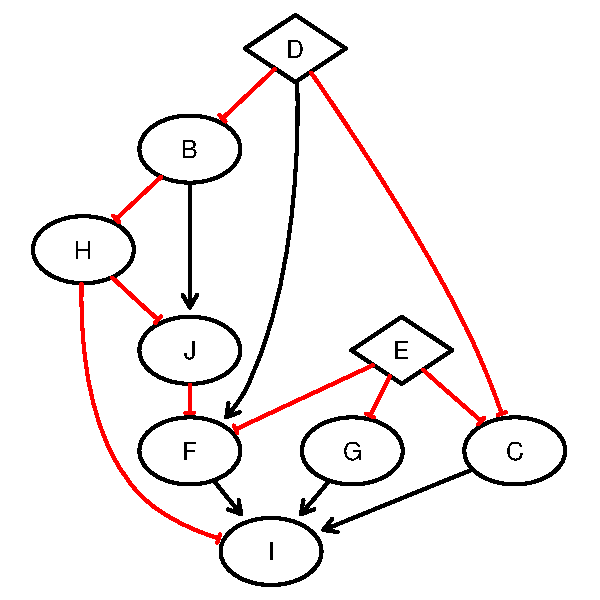
\includegraphics[width=0.4\linewidth]{figure/plotpkn-1} 

}



\end{knitrout}
In the next step we convert the dnf object into a PKN and extend it to a Boolean hyper-graph, which includes all functions allowed by the PKN.
\begin{knitrout}
\definecolor{shadecolor}{rgb}{0.969, 0.969, 0.969}\color{fgcolor}\begin{kframe}
\begin{alltt}
\hlstd{sifMatrix} \hlkwb{<-} \hlkwa{NULL}

\hlkwa{for} \hlstd{(i} \hlkwa{in} \hlstd{dnf) \{}
  \hlstd{inputs2} \hlkwb{<-} \hlkwd{unique}\hlstd{(}\hlkwd{unlist}\hlstd{(}\hlkwd{strsplit}\hlstd{(}\hlkwd{gsub}\hlstd{(}\hlstr{"=.*"}\hlstd{,} \hlstr{""}\hlstd{, i),} \hlstr{"="}\hlstd{)))}
  \hlstd{output} \hlkwb{<-} \hlkwd{unique}\hlstd{(}\hlkwd{gsub}\hlstd{(}\hlstr{".*="}\hlstd{,} \hlstr{""}\hlstd{, i))}
  \hlkwa{for} \hlstd{(j} \hlkwa{in} \hlstd{inputs2) \{}
    \hlstd{j2} \hlkwb{<-} \hlkwd{gsub}\hlstd{(}\hlstr{"!"}\hlstd{,} \hlstr{""}\hlstd{, j)}
    \hlkwa{if} \hlstd{(j} \hlopt \hlstd{j2) \{}
      \hlstd{sifMatrix} \hlkwb{<-} \hlkwd{rbind}\hlstd{(sifMatrix,} \hlkwd{c}\hlstd{(j,} \hlnum{1}\hlstd{, output))}
    \hlstd{\}} \hlkwa{else} \hlstd{\{}
      \hlstd{sifMatrix} \hlkwb{<-} \hlkwd{rbind}\hlstd{(sifMatrix,} \hlkwd{c}\hlstd{(j2,} \hlopt{-}\hlnum{1}\hlstd{, output))}
    \hlstd{\}}
  \hlstd{\}}
\hlstd{\}}
\hlkwd{write.table}\hlstd{(sifMatrix,} \hlkwc{file} \hlstd{=} \hlstr{"temp.sif"}\hlstd{,} \hlkwc{sep} \hlstd{=} \hlstr{"\textbackslash{}t"}\hlstd{,} \hlkwc{row.names} \hlstd{=} \hlnum{FALSE}\hlstd{,} \hlkwc{col.names} \hlstd{=} \hlnum{FALSE}\hlstd{,} \hlkwc{quote} \hlstd{=} \hlnum{FALSE}\hlstd{)}
\hlstd{PKN} \hlkwb{<-} \hlkwd{readSIF}\hlstd{(}\hlstr{"temp.sif"}\hlstd{)}
\hlcom{## unlink("temp.sif")}

\hlcom{## create dummy metainformation:}
\hlstd{CNOlist} \hlkwb{<-} \hlkwd{dummyCNOlist}\hlstd{(}\hlkwc{stimuli} \hlstd{= stimuli,} \hlkwc{inhibitors} \hlstd{= inhibitors,} \hlkwc{maxStim} \hlstd{=} \hlnum{2}\hlstd{,} \hlkwc{maxInhibit} \hlstd{=} \hlnum{1}\hlstd{,} \hlkwc{signals} \hlstd{=} \hlkwa{NULL}\hlstd{)}

\hlcom{## extend the model:}
\hlstd{model} \hlkwb{<-} \hlkwd{preprocessing}\hlstd{(CNOlist, PKN,} \hlkwc{maxInputsPerGate}\hlstd{=}\hlnum{100}\hlstd{)}
\end{alltt}
\begin{verbatim}
## [1] "The following species are measured: B, C, D, E, F, G, H, I, J"
## [1] "The following species are stimulated: D, E"
## [1] "The following species are inhibited: B, C, F, G, H, I, J"
## [1] "The following species are not observable and/or not controllable: "
\end{verbatim}
\end{kframe}
\end{knitrout}
We suggest to take a look at the sif file. In future analyses it is easier to just provide a suitable sif file for the investigated pathway.

In a real world application the underlaying real ground truth network (GTN) is not known. However in our toy example we define one.
\begin{knitrout}
\definecolor{shadecolor}{rgb}{0.969, 0.969, 0.969}\color{fgcolor}\begin{kframe}
\begin{alltt}
\hlcom{## define a bitstring denoting the present and absent edges:}
\hlstd{bString} \hlkwb{<-} \hlkwd{absorption}\hlstd{(}\hlkwd{sample}\hlstd{(}\hlkwd{c}\hlstd{(}\hlnum{0}\hlstd{,}\hlnum{1}\hlstd{),} \hlkwd{length}\hlstd{(model}\hlopt{$}\hlstd{reacID),} \hlkwc{replace} \hlstd{= T), model)}

\hlcom{## simulate S-gene states for all possible conditions:}
\hlstd{steadyState} \hlkwb{<-} \hlstd{steadyState2} \hlkwb{<-} \hlkwd{simulateStatesRecursive}\hlstd{(CNOlist, model, bString)}

\hlcom{## we find constitutively active S-genes with the folloing:}
\hlstd{steadyState2[,} \hlkwd{grep}\hlstd{(}\hlkwd{paste}\hlstd{(inhibitors,} \hlkwc{collapse} \hlstd{=} \hlstr{"|"}\hlstd{),} \hlkwd{colnames}\hlstd{(steadyState2))]} \hlkwb{<-} \hlstd{steadyState2[,} \hlkwd{grep}\hlstd{(}\hlkwd{paste}\hlstd{(inhibitors,} \hlkwc{collapse} \hlstd{=} \hlstr{"|"}\hlstd{),} \hlkwd{colnames}\hlstd{(steadyState2))]} \hlopt{+} \hlstd{CNOlist}\hlopt{@}\hlkwc{inhibitors}

\hlcom{## this while loop makes sure we get a gtn which actually affects all vertices and no vertices are constitutively active (not necessary):}
\hlkwa{while}\hlstd{(}\hlkwd{any}\hlstd{(}\hlkwd{apply}\hlstd{(steadyState,} \hlnum{2}\hlstd{, sd)} \hlopt{==} \hlnum{0}\hlstd{)} \hlopt{|} \hlkwd{any}\hlstd{(}\hlkwd{apply}\hlstd{(steadyState2,} \hlnum{2}\hlstd{, sd)} \hlopt{==} \hlnum{0}\hlstd{)) \{}

  \hlstd{bString} \hlkwb{<-} \hlkwd{absorption}\hlstd{(}\hlkwd{sample}\hlstd{(}\hlkwd{c}\hlstd{(}\hlnum{0}\hlstd{,}\hlnum{1}\hlstd{),} \hlkwd{length}\hlstd{(model}\hlopt{$}\hlstd{reacID),} \hlkwc{replace} \hlstd{= T), model)}

  \hlstd{steadyState} \hlkwb{<-} \hlstd{steadyState2} \hlkwb{<-} \hlkwd{simulateStatesRecursive}\hlstd{(CNOlist, model, bString)}

  \hlstd{steadyState2[,} \hlkwd{grep}\hlstd{(}\hlkwd{paste}\hlstd{(inhibitors,} \hlkwc{collapse} \hlstd{=} \hlstr{"|"}\hlstd{),} \hlkwd{colnames}\hlstd{(steadyState2))]} \hlkwb{<-} \hlstd{steadyState2[,} \hlkwd{grep}\hlstd{(}\hlkwd{paste}\hlstd{(inhibitors,} \hlkwc{collapse} \hlstd{=} \hlstr{"|"}\hlstd{),} \hlkwd{colnames}\hlstd{(steadyState2))]} \hlopt{+} \hlstd{CNOlist}\hlopt{@}\hlkwc{inhibitors}

\hlstd{\}}
\end{alltt}
\end{kframe}
\end{knitrout}
The following figure shows our random GTN, which is a subset of the complete search space (model based on the PKN).
\begin{knitrout}
\definecolor{shadecolor}{rgb}{0.969, 0.969, 0.969}\color{fgcolor}\begin{kframe}
\begin{alltt}
\hlkwd{plotDnf}\hlstd{(model}\hlopt{$}\hlstd{reacID[}\hlkwd{as.logical}\hlstd{(bString)],} \hlkwc{stimuli} \hlstd{= stimuli)}
\end{alltt}
\begin{verbatim}
## A graphNEL graph with directed edges
## Number of Nodes = 11 
## Number of Edges = 14
\end{verbatim}
\end{kframe}

{\centering 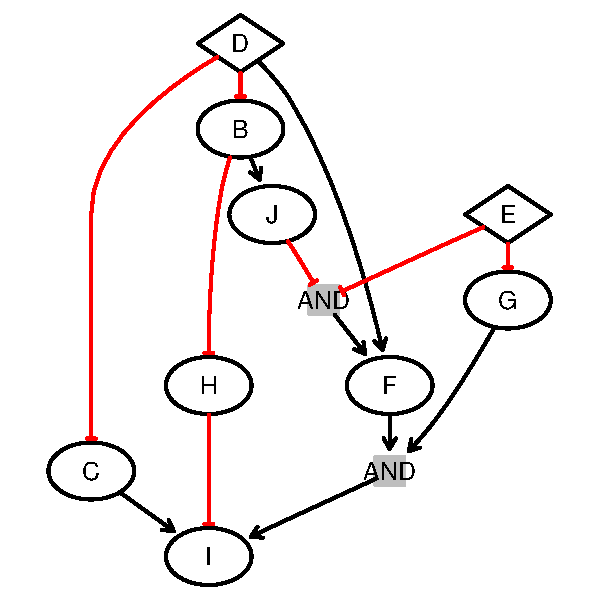
\includegraphics[width=0.4\linewidth]{figure/plotgtn-1} 

}



\end{knitrout}
We now use this GTN to simulate data.
\begin{knitrout}
\definecolor{shadecolor}{rgb}{0.969, 0.969, 0.969}\color{fgcolor}\begin{kframe}
\begin{alltt}
\hlcom{## the expression data with 10 E-genes for each S-gene and 3 replicates (not used):}
\hlstd{exprs} \hlkwb{<-} \hlkwd{t}\hlstd{(steadyState)[}\hlkwd{rep}\hlstd{(}\hlnum{1}\hlopt{:}\hlkwd{ncol}\hlstd{(steadyState),} \hlnum{10}\hlstd{),} \hlkwd{rep}\hlstd{(}\hlnum{1}\hlopt{:}\hlkwd{nrow}\hlstd{(steadyState),} \hlnum{3}\hlstd{)]}

\hlcom{## we calculate the foldchanges or expected S-gene response scheme (ERS) between certain condtion (e.g. control vs stimulation):}
\hlstd{ERS} \hlkwb{<-} \hlkwd{computeFc}\hlstd{(CNOlist,} \hlkwd{t}\hlstd{(steadyState))}

\hlcom{# the next step reduces the ERS to a sensible set of comparisons; e.g. we do not want to compare stimuli vs inhibition, but stimuli vs (stimuli,inhibition):}
\hlstd{stimuli.pairs} \hlkwb{<-} \hlkwd{apply}\hlstd{(}\hlkwd{apply}\hlstd{(}\hlkwd{expand.grid}\hlstd{(stimuli, stimuli),} \hlkwd{c}\hlstd{(}\hlnum{1}\hlstd{,}\hlnum{2}\hlstd{), as.character),} \hlnum{1}\hlstd{, paste,} \hlkwc{collapse} \hlstd{=} \hlstr{"_"}\hlstd{)}

\hlcom{## this is the usual setup, but "computeFc" calculates a lot more contrasts, which can also be used if preferred:}
\hlstd{ERS} \hlkwb{<-} \hlstd{ERS[,} \hlkwd{grep}\hlstd{(}\hlkwd{paste}\hlstd{(}\hlkwd{c}\hlstd{(}\hlkwd{paste}\hlstd{(}\hlstr{"Ctrl_vs_"}\hlstd{,} \hlkwd{c}\hlstd{(stimuli, inhibitors),} \hlkwc{sep} \hlstd{=} \hlstr{""}\hlstd{),} \hlkwd{paste}\hlstd{(stimuli,} \hlstr{"_vs_"}\hlstd{, stimuli,} \hlstr{"_"}\hlstd{,} \hlkwd{rep}\hlstd{(inhibitors,} \hlkwc{each} \hlstd{=} \hlkwd{length}\hlstd{(stimuli)),} \hlkwc{sep} \hlstd{=} \hlstr{""}\hlstd{),} \hlkwd{paste}\hlstd{(stimuli.pairs,} \hlstr{"_vs_"}\hlstd{, stimuli.pairs,} \hlstr{"_"}\hlstd{,} \hlkwd{rep}\hlstd{(inhibitors,} \hlkwc{each} \hlstd{=} \hlkwd{length}\hlstd{(stimuli.pairs)),} \hlkwc{sep} \hlstd{=} \hlstr{""}\hlstd{)),} \hlkwc{collapse} \hlstd{=} \hlstr{"|"}\hlstd{),} \hlkwd{colnames}\hlstd{(ERS))]}

\hlcom{## same as before with the expression values, we have 10 E-genes each and 3 replicates:}
\hlstd{fc} \hlkwb{<-} \hlstd{ERS[}\hlkwd{rep}\hlstd{(}\hlnum{1}\hlopt{:}\hlkwd{nrow}\hlstd{(ERS),} \hlnum{10}\hlstd{),} \hlkwd{rep}\hlstd{(}\hlnum{1}\hlopt{:}\hlkwd{ncol}\hlstd{(ERS),} \hlnum{3}\hlstd{)]}

\hlcom{## we add some Gaussian noise:}
\hlstd{fc} \hlkwb{<-} \hlstd{fc} \hlopt{+} \hlkwd{rnorm}\hlstd{(}\hlkwd{length}\hlstd{(fc),} \hlnum{0}\hlstd{,} \hlnum{1}\hlstd{)}

\hlcom{## some E-genes are negative regulated, hence we flip their foldchanges:}
\hlstd{flip} \hlkwb{<-} \hlkwd{sample}\hlstd{(}\hlnum{1}\hlopt{:}\hlkwd{nrow}\hlstd{(fc),} \hlkwd{floor}\hlstd{(}\hlnum{0.33}\hlopt{*}\hlkwd{row}\hlstd{(fc)))}
\hlstd{fc[flip, ]} \hlkwb{<-} \hlstd{fc[flip, ]}\hlopt{*}\hlstd{(}\hlopt{-}\hlnum{1}\hlstd{)}

\hlcom{## don't forget to set rownames (usually gene ids)}
\hlkwd{rownames}\hlstd{(fc)} \hlkwb{<-} \hlkwd{paste}\hlstd{(}\hlkwd{rownames}\hlstd{(fc),} \hlnum{1}\hlopt{:}\hlkwd{nrow}\hlstd{(fc),} \hlkwc{sep} \hlstd{=} \hlstr{"_"}\hlstd{)}
\hlkwd{print}\hlstd{(fc[}\hlnum{1}\hlopt{:}\hlnum{6}\hlstd{,} \hlkwd{c}\hlstd{(}\hlnum{1}\hlopt{:}\hlnum{3}\hlstd{,(}\hlkwd{ncol}\hlstd{(fc)}\hlopt{-}\hlnum{2}\hlstd{)}\hlopt{:}\hlkwd{ncol}\hlstd{(fc))])}
\end{alltt}
\begin{verbatim}
##       Ctrl_vs_F  Ctrl_vs_G   Ctrl_vs_J D_E_vs_D_E_H D_E_vs_D_E_C D_E_vs_D_E_I
## B_1  0.57024784  0.2421169 -0.71445606   -0.9938059   -1.6165289   -1.4213850
## C_2 -1.70109567  1.0961857 -0.09249841   -0.1175367   -1.4843078   -1.6976438
## D_3 -1.14748014 -1.7113624  1.38419998   -0.3473269   -0.3694678   -0.8627585
## E_4  1.17990384  0.6426374 -0.24184371    0.5973451   -0.1545769   -0.4779243
## F_5 -1.19006930 -1.1619101  1.85210676    0.1237633   -1.8796660   -0.6152921
## G_6  0.07252035 -0.6971871  1.24181503   -1.8159441    0.5004976   -1.4542246
\end{verbatim}
\end{kframe}
\end{knitrout}
B-NEM uses differential expression between experiments to infer the
pathway logics. For example look at the colnames of fc (=foldchanges
of E-genes (rows)) and remember that D, E are our
stimulated S-genes and the rest possibly inhibited. Thus in the first
column of fc we have the contrast F $-$ control. In the control no S-genes are perturbed.

We search for the GTN in our restricted network space. Each network is a sub-graph of the full hyper-graph model\$reacID. We initialise the search with a starting network and greedily search the neighbourhood.

\begin{knitrout}
\definecolor{shadecolor}{rgb}{0.969, 0.969, 0.969}\color{fgcolor}\begin{kframe}
\begin{alltt}
\hlcom{## start with empty graph:}
\hlstd{initBstring} \hlkwb{<-} \hlkwd{reduceGraph}\hlstd{(}\hlkwd{rep}\hlstd{(}\hlnum{0}\hlstd{,} \hlkwd{length}\hlstd{(model}\hlopt{$}\hlstd{reacID)), model, CNOlist)}
\hlcom{## initBstring <- reduceGraph(rep(1, length(model$reacID)), model, CNOlist)}

\hlcom{## paralellize for several threads on one machine or multiple machines. See package "snowfall" for details.}
\hlstd{parallel} \hlkwb{<-} \hlnum{2} \hlcom{# list(c(4,16,8,2), c("machine1", "machine2", "machine3", "machine4"))}

\hlcom{## greedy search:}
\hlstd{greedy} \hlkwb{<-} \hlkwd{bnem}\hlstd{(}\hlkwc{search} \hlstd{=} \hlstr{"greedy"}\hlstd{,}
            \hlkwc{fc}\hlstd{=fc,}
            \hlkwc{exprs}\hlstd{=exprs,} \hlcom{# not used, if fc is defined}
            \hlkwc{CNOlist}\hlstd{=CNOlist,}
            \hlkwc{model}\hlstd{=model,}
            \hlkwc{parallel}\hlstd{=parallel,}
            \hlkwc{initBstring}\hlstd{=initBstring,}
            \hlkwc{draw} \hlstd{=} \hlnum{FALSE}\hlstd{,}
            \hlkwc{verbose} \hlstd{=} \hlnum{FALSE}\hlstd{,}
            \hlkwc{maxSteps} \hlstd{=} \hlnum{Inf}
            \hlstd{)}
\end{alltt}


{\ttfamily\noindent\itshape\color{messagecolor}{\#\# snowfall 1.84-6.1 initialized (using snow 0.4-1): parallel execution on 2 CPUs.}}\begin{verbatim}
## Library CellNOptR loaded.
\end{verbatim}


{\ttfamily\noindent\itshape\color{messagecolor}{\#\# Library CellNOptR loaded in cluster.}}\begin{verbatim}
## Library bnem loaded.
\end{verbatim}


{\ttfamily\noindent\itshape\color{messagecolor}{\#\# Library bnem loaded in cluster.}}

{\ttfamily\noindent\itshape\color{messagecolor}{\#\# \\\#\# Stopping cluster}}\begin{alltt}
\hlstd{resString} \hlkwb{<-} \hlstd{greedy}\hlopt{$}\hlstd{bString}
\end{alltt}
\end{kframe}
\end{knitrout}
We can now take a look at the efficiency of the search algorithm with sensitivity and specificity of the optimal found network and the accuracy of its ERS (similar to the truth table). Since several network produce the same ERS, the found hyper-graph can differ from the GTN and still be $100\%$ accurate.
\begin{knitrout}
\definecolor{shadecolor}{rgb}{0.969, 0.969, 0.969}\color{fgcolor}\begin{kframe}
\begin{alltt}
\hlkwd{par}\hlstd{(}\hlkwc{mfrow}\hlstd{=}\hlkwd{c}\hlstd{(}\hlnum{1}\hlstd{,}\hlnum{2}\hlstd{))}

\hlcom{## GTN:}
\hlkwd{plotDnf}\hlstd{(model}\hlopt{$}\hlstd{reacID[}\hlkwd{as.logical}\hlstd{(bString)],} \hlkwc{main} \hlstd{=} \hlstr{"GTN"}\hlstd{,} \hlkwc{stimuli} \hlstd{= stimuli)}
\end{alltt}
\begin{verbatim}
## A graphNEL graph with directed edges
## Number of Nodes = 11 
## Number of Edges = 14
\end{verbatim}
\begin{alltt}
\hlcom{## optimum found:}
\hlkwd{plotDnf}\hlstd{(model}\hlopt{$}\hlstd{reacID[}\hlkwd{as.logical}\hlstd{(resString)],} \hlkwc{main} \hlstd{=} \hlstr{"greedy optimum"}\hlstd{,} \hlkwc{stimuli} \hlstd{= stimuli)}
\end{alltt}
\begin{verbatim}
## A graphNEL graph with directed edges
## Number of Nodes = 11 
## Number of Edges = 14
\end{verbatim}
\end{kframe}

{\centering 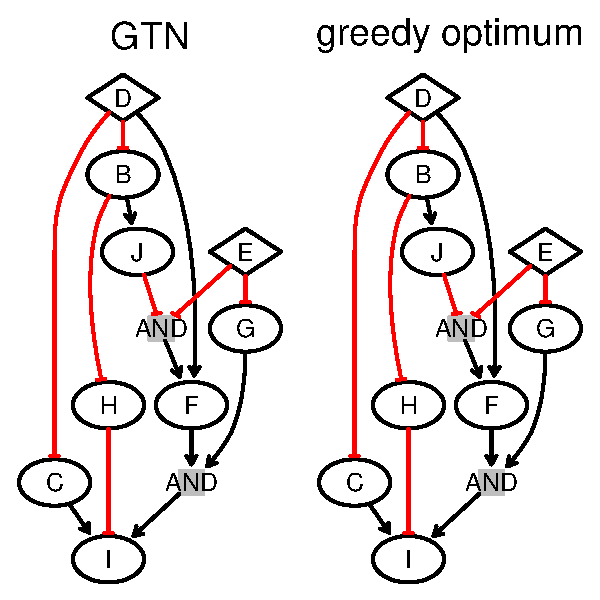
\includegraphics[width=0.4\linewidth]{figure/plotresult-1} 

}



\end{knitrout}
\begin{knitrout}
\definecolor{shadecolor}{rgb}{0.969, 0.969, 0.969}\color{fgcolor}\begin{kframe}
\begin{alltt}
\hlcom{## hyper-edge sensitivity and specificity:}
\hlkwd{print}\hlstd{(}\hlkwd{sum}\hlstd{(bString} \hlopt{==} \hlnum{1} \hlopt{&} \hlstd{resString} \hlopt{==} \hlnum{1}\hlstd{)}\hlopt{/}\hlstd{(}\hlkwd{sum}\hlstd{(bString} \hlopt{==} \hlnum{1} \hlopt{&} \hlstd{resString} \hlopt{==} \hlnum{1}\hlstd{)} \hlopt{+} \hlkwd{sum}\hlstd{(bString} \hlopt{==} \hlnum{1} \hlopt{&} \hlstd{resString} \hlopt{==} \hlnum{0}\hlstd{)))}
\end{alltt}
\begin{verbatim}
## [1] 1
\end{verbatim}
\begin{alltt}
\hlkwd{print}\hlstd{(}\hlkwd{sum}\hlstd{(bString} \hlopt{==} \hlnum{0} \hlopt{&} \hlstd{resString} \hlopt{==} \hlnum{0}\hlstd{)}\hlopt{/}\hlstd{(}\hlkwd{sum}\hlstd{(bString} \hlopt{==} \hlnum{0} \hlopt{&} \hlstd{resString} \hlopt{==} \hlnum{0}\hlstd{)} \hlopt{+} \hlkwd{sum}\hlstd{(bString} \hlopt{==} \hlnum{0} \hlopt{&} \hlstd{resString} \hlopt{==} \hlnum{1}\hlstd{)))}
\end{alltt}
\begin{verbatim}
## [1] 1
\end{verbatim}
\begin{alltt}
\hlcom{## accuracy of expected response scheme from learned network should be high even though the network can look different:}
\hlstd{ERS.res} \hlkwb{<-} \hlkwd{computeFc}\hlstd{(CNOlist,} \hlkwd{t}\hlstd{(}\hlkwd{simulateStatesRecursive}\hlstd{(CNOlist, model, resString)))}
\hlstd{ERS.res} \hlkwb{<-} \hlstd{ERS.res[,} \hlkwd{which}\hlstd{(}\hlkwd{colnames}\hlstd{(ERS.res)} \hlopt \hlkwd{colnames}\hlstd{(ERS))]}
\hlkwd{print}\hlstd{(}\hlkwd{sum}\hlstd{(ERS.res} \hlopt{==} \hlstd{ERS)}\hlopt{/}\hlkwd{length}\hlstd{(ERS))}
\end{alltt}
\begin{verbatim}
## [1] 1
\end{verbatim}
\end{kframe}
\end{knitrout}
In our seeded example 2574 the optimum network is indeed the GTN. If you set the alternative seed at the beginning, neither the network nor the correct ERS is found with the empty network at the start. If you start with the PKN, the ERS is resolved completely while the network is still not the GTN. Thus the GTN and the optimum are equivalent, but the GTN is larger and thus not preferred.

After optimization you can look at the data and how well your networks explains the E-genes. The lower the score the better the fit.

\begin{knitrout}
\definecolor{shadecolor}{rgb}{0.969, 0.969, 0.969}\color{fgcolor}\begin{kframe}
\begin{alltt}
\hlstd{fitinfo} \hlkwb{<-} \hlkwd{validateGraph}\hlstd{(CNOlist,} \hlkwc{fc}\hlstd{=fc,} \hlkwc{exprs}\hlstd{=exprs,} \hlkwc{model} \hlstd{= model,} \hlkwc{bString} \hlstd{= resString,} \hlkwc{Sgene} \hlstd{=} \hlnum{1}\hlstd{,} \hlkwc{Egenes} \hlstd{=} \hlnum{1000}\hlstd{,} \hlkwc{cexRow} \hlstd{=} \hlnum{0.8}\hlstd{,} \hlkwc{cexCol} \hlstd{=} \hlnum{0.7}\hlstd{,} \hlkwc{xrot} \hlstd{=} \hlnum{45}\hlstd{,} \hlkwc{disc} \hlstd{=} \hlnum{0}\hlstd{,} \hlkwc{Colv} \hlstd{= T,} \hlkwc{Rowv} \hlstd{= T,} \hlkwc{dendrogram} \hlstd{=} \hlstr{"both"}\hlstd{,} \hlkwc{bordercol} \hlstd{=} \hlstr{"lightgrey"}\hlstd{,} \hlkwc{aspect} \hlstd{=} \hlstr{"iso"}\hlstd{,} \hlkwc{sub} \hlstd{=} \hlstr{""}\hlstd{)}
\end{alltt}
\begin{verbatim}
## [1] "1.B: 13"
## [1] "Activated: 6"
## [1] "Inhibited: 7"
## [1] "Summary Score:"
##    Min. 1st Qu.  Median    Mean 3rd Qu.    Max. 
## -0.5542 -0.4978 -0.4754 -0.4542 -0.4466 -0.2345 
## [1] "Unique genes used: 90 (100 %)"
## [1] "Duplicated genes: 0"
## [1] "Overall fit:"
##    Min. 1st Qu.  Median    Mean 3rd Qu.    Max. 
## -0.6368 -0.5190 -0.4505 -0.4327 -0.3601 -0.1497
\end{verbatim}
\end{kframe}

{\centering 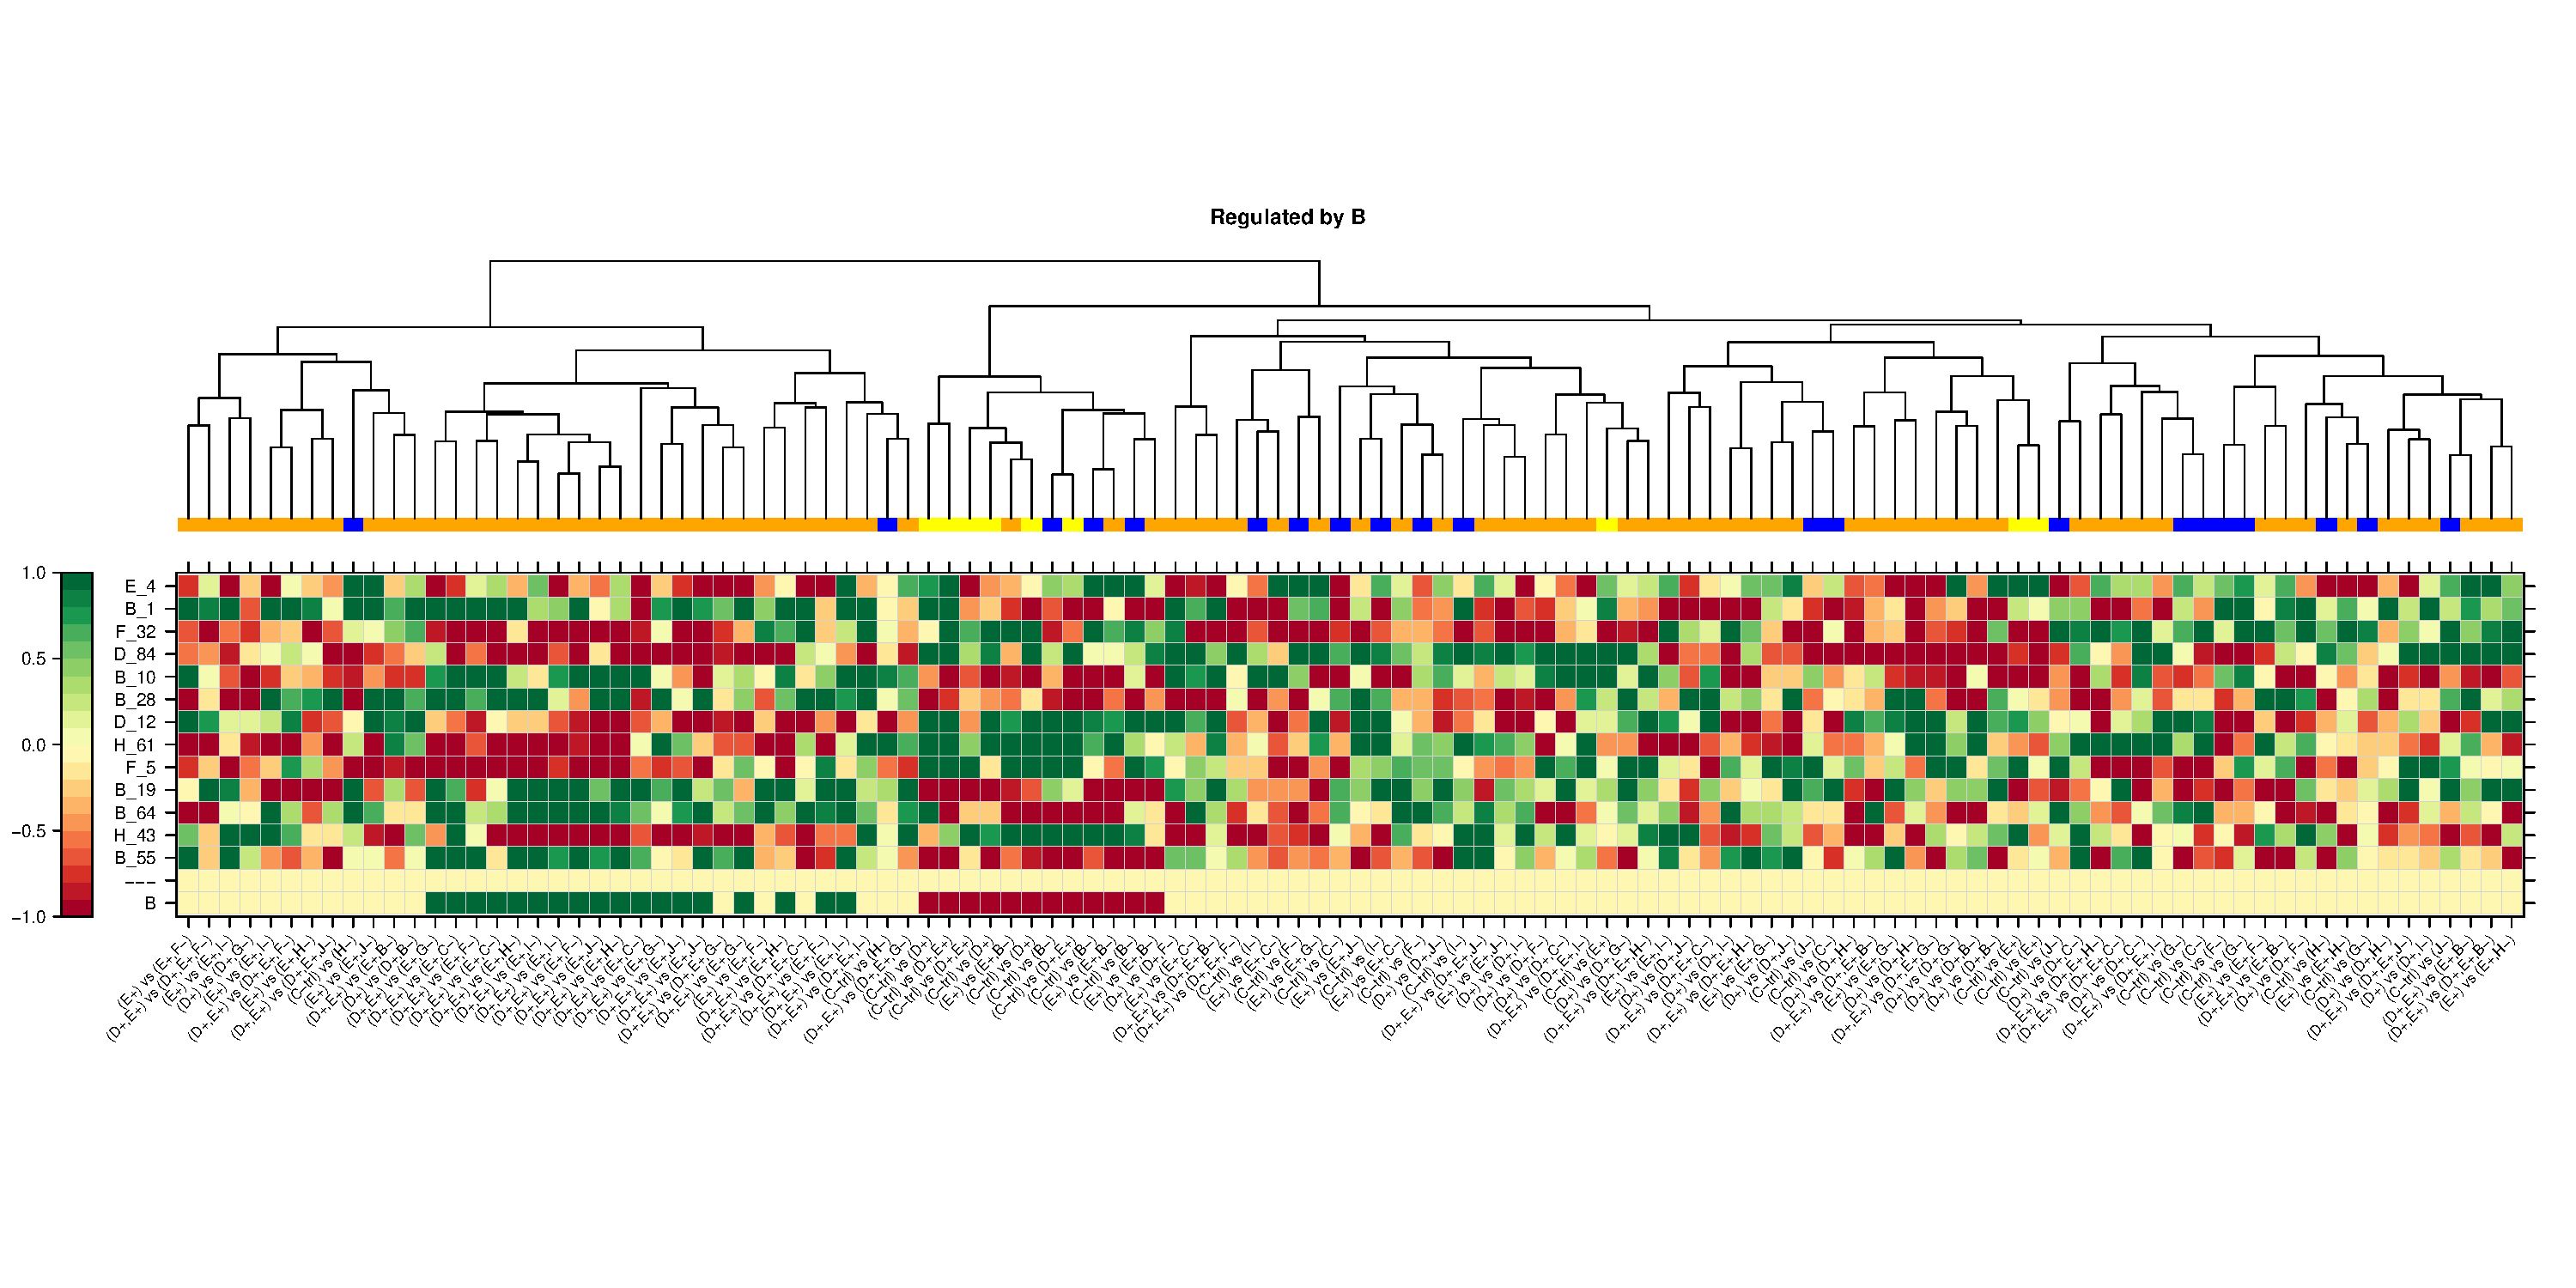
\includegraphics[width=1.0\linewidth]{figure/visualfit-1} 

}



\end{knitrout}

The bottom row shows the ERS of S-gene B and the other rows show the observed response scheme (ORS) of the B-regulated E-genes. Even though the Gaussian noise makes the data look almost random, we still found the GTN.
Alternatively to the greedy neightbourhood search a genetic algorithm and exhaustive search are also available. The exhaustive search is not recommended for search spaces with more than 20 hyper-edges.


\begin{knitrout}
\definecolor{shadecolor}{rgb}{0.969, 0.969, 0.969}\color{fgcolor}\begin{kframe}
\begin{alltt}
\hlcom{## genetic algorithm:}
\hlstd{genetic} \hlkwb{<-} \hlkwd{bnem}\hlstd{(}\hlkwc{search} \hlstd{=} \hlstr{"genetic"}\hlstd{,}
           \hlkwc{fc}\hlstd{=fc,}
           \hlkwc{exprs}\hlstd{=exprs,}
           \hlkwc{parallel} \hlstd{= parallel,}
           \hlkwc{CNOlist}\hlstd{=CNOlist,}
           \hlkwc{model}\hlstd{=model,}
           \hlkwc{initBstring}\hlstd{=initBstring,}
           \hlkwc{popSize} \hlstd{=} \hlnum{10}\hlstd{,}
           \hlkwc{stallGenMax} \hlstd{=} \hlnum{10}\hlstd{,}
           \hlkwc{graph} \hlstd{=} \hlnum{FALSE}\hlstd{,}
           \hlkwc{verbose} \hlstd{=} \hlnum{FALSE}
           \hlstd{)}
\end{alltt}


{\ttfamily\noindent\itshape\color{messagecolor}{\#\# snowfall 1.84-6.1 initialized (using snow 0.4-1): parallel execution on 2 CPUs.}}\begin{verbatim}
## Library CellNOptR loaded.
\end{verbatim}


{\ttfamily\noindent\itshape\color{messagecolor}{\#\# Library CellNOptR loaded in cluster.}}\begin{verbatim}
## Library bnem loaded.
\end{verbatim}


{\ttfamily\noindent\itshape\color{messagecolor}{\#\# Library bnem loaded in cluster.}}

{\ttfamily\noindent\itshape\color{messagecolor}{\#\# \\\#\# Stopping cluster}}\begin{alltt}
\hlstd{resString} \hlkwb{<-} \hlstd{genetic}\hlopt{$}\hlstd{bString}
\end{alltt}
\end{kframe}
\end{knitrout}
\begin{knitrout}
\definecolor{shadecolor}{rgb}{0.969, 0.969, 0.969}\color{fgcolor}\begin{kframe}
\begin{alltt}
\hlcom{## ## exhaustive search:}
\hlcom{## exhaustive <- bnem(search = "exhaustive",}
\hlcom{##            parallel = parallel,}
\hlcom{##            CNOlist=CNOlist,}
\hlcom{##            fc=fc,}
\hlcom{##            exprs=exprs,}
\hlcom{##            model=model}
\hlcom{##            )}

\hlcom{## resString <- exRun$bString}
\end{alltt}
\end{kframe}
\end{knitrout}

\section*{Stimulated and inhibited S-genes can overlap}
In this section we show how to use B-NEM when stimuli and inhibitors overlap. For this we allow the PKN to have cycles, but no repression, because repression can lead to an unresolvable ERS. See Pirkl et al., 2016 for details.

\begin{knitrout}
\definecolor{shadecolor}{rgb}{0.969, 0.969, 0.969}\color{fgcolor}\begin{kframe}
\begin{alltt}
\hlcom{## we do not force a DAG but do not allow repression:}
\hlstd{dnf} \hlkwb{<-} \hlkwd{randomDnf}\hlstd{(}\hlnum{10}\hlstd{,} \hlkwc{max.edges} \hlstd{=} \hlnum{25}\hlstd{,} \hlkwc{max.edge.size} \hlstd{=} \hlnum{1}\hlstd{,} \hlkwc{dag} \hlstd{= F,} \hlkwc{negation} \hlstd{= F)}
\hlstd{cues} \hlkwb{<-} \hlkwd{sort}\hlstd{(}\hlkwd{unique}\hlstd{(}\hlkwd{gsub}\hlstd{(}\hlstr{"!"}\hlstd{,} \hlstr{""}\hlstd{,} \hlkwd{unlist}\hlstd{(}\hlkwd{strsplit}\hlstd{(}\hlkwd{unlist}\hlstd{(}\hlkwd{strsplit}\hlstd{(dnf,} \hlstr{"="}\hlstd{)),} \hlstr{"\textbackslash{}\textbackslash{}+"}\hlstd{)))))}
\hlstd{inputs} \hlkwb{<-} \hlkwd{unique}\hlstd{(}\hlkwd{unlist}\hlstd{(}\hlkwd{strsplit}\hlstd{(}\hlkwd{gsub}\hlstd{(}\hlstr{"!"}\hlstd{,} \hlstr{""}\hlstd{,} \hlkwd{gsub}\hlstd{(}\hlstr{"=.*"}\hlstd{,} \hlstr{""}\hlstd{, dnf)),} \hlstr{"="}\hlstd{)))}
\hlstd{outputs} \hlkwb{<-} \hlkwd{unique}\hlstd{(}\hlkwd{gsub}\hlstd{(}\hlstr{".*="}\hlstd{,} \hlstr{""}\hlstd{, dnf))}
\hlstd{stimuli} \hlkwb{<-} \hlkwd{c}\hlstd{(inputs[}\hlkwd{which}\hlstd{(}\hlopt{!}\hlstd{(inputs} \hlopt \hlstd{outputs))], cues[}\hlkwd{sample}\hlstd{(}\hlnum{1}\hlopt{:}\hlkwd{length}\hlstd{(cues),} \hlnum{2}\hlstd{)])}
\hlstd{inhibitors} \hlkwb{<-} \hlstd{cues}
\end{alltt}
\end{kframe}
\end{knitrout}

Now we look for stimuli which are also inhibited. For those we add additional stimuli S-genes. The stimuli S-gene (parent) and the inhibitor S-gene (child) are connected by a positive edge.

\begin{knitrout}
\definecolor{shadecolor}{rgb}{0.969, 0.969, 0.969}\color{fgcolor}\begin{kframe}
\begin{alltt}
\hlstd{both} \hlkwb{<-} \hlstd{stimuli[}\hlkwd{which}\hlstd{(stimuli} \hlopt \hlstd{inhibitors)]}
\hlkwa{for} \hlstd{(i} \hlkwa{in} \hlstd{both) \{}
  \hlstd{dnf} \hlkwb{<-} \hlkwd{gsub}\hlstd{(i,} \hlkwd{paste}\hlstd{(i,} \hlstr{"inhibit"}\hlstd{,} \hlkwc{sep} \hlstd{=} \hlstr{""}\hlstd{), dnf)}
  \hlstd{dnf} \hlkwb{<-} \hlkwd{c}\hlstd{(dnf,} \hlkwd{paste}\hlstd{(i,} \hlstr{"stim="}\hlstd{, i,} \hlstr{"inhibit"}\hlstd{,} \hlkwc{sep} \hlstd{=} \hlstr{""}\hlstd{))}
  \hlstd{stimuli} \hlkwb{<-} \hlkwd{gsub}\hlstd{(i,} \hlkwd{paste}\hlstd{(i,} \hlstr{"stim"}\hlstd{,} \hlkwc{sep} \hlstd{=} \hlstr{""}\hlstd{), stimuli)}
  \hlstd{inhibitors}  \hlkwb{<-} \hlkwd{gsub}\hlstd{(i,} \hlkwd{paste}\hlstd{(i,} \hlstr{"inhibit"}\hlstd{,} \hlkwc{sep} \hlstd{=} \hlstr{""}\hlstd{), inhibitors)}
\hlstd{\}}
\end{alltt}
\end{kframe}
\end{knitrout}

The next figure shows the cyclic PKN with extra stimuli S-genes. Notice, this way the inhibition of the S-genes overrules the stimulation.

\begin{knitrout}
\definecolor{shadecolor}{rgb}{0.969, 0.969, 0.969}\color{fgcolor}\begin{kframe}
\begin{alltt}
\hlkwd{plotDnf}\hlstd{(dnf,} \hlkwc{stimuli} \hlstd{= stimuli)}
\end{alltt}
\begin{verbatim}
## A graphNEL graph with directed edges
## Number of Nodes = 13 
## Number of Edges = 28
\end{verbatim}
\end{kframe}

{\centering 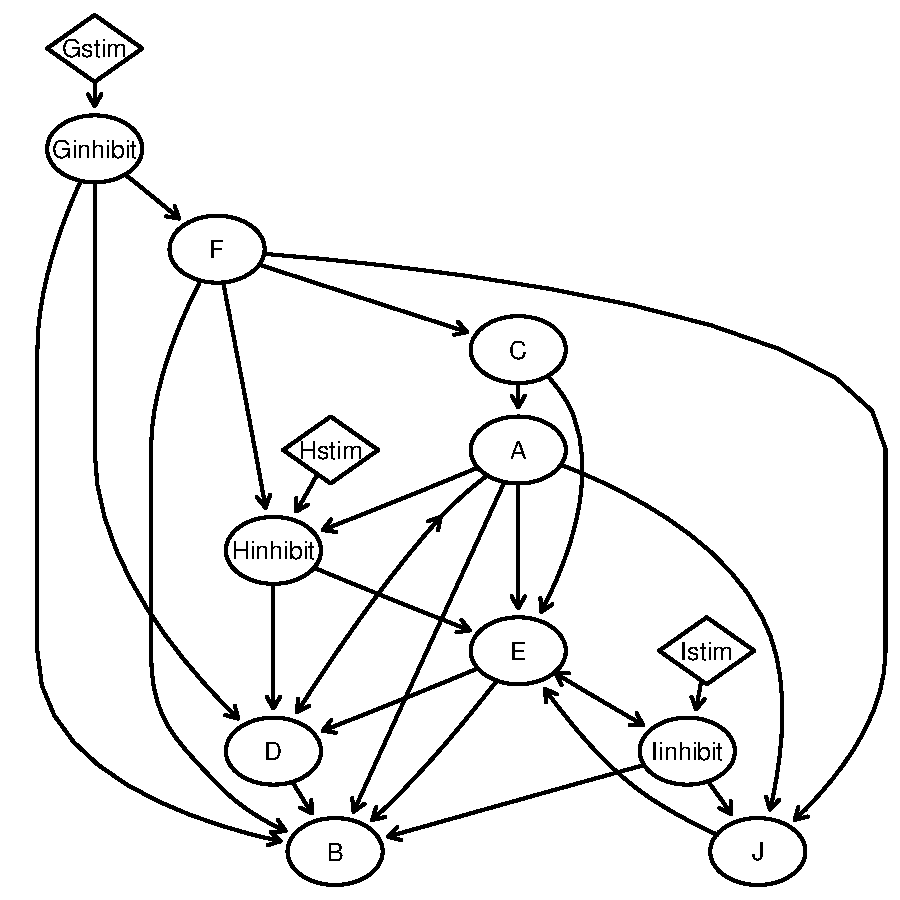
\includegraphics[width=0.6\linewidth]{figure/plotpkn2-1} 

}



\end{knitrout}

Similar to before we create the full network search space, draw a GTN, simulate data and search for the optimal network.

\begin{knitrout}
\definecolor{shadecolor}{rgb}{0.969, 0.969, 0.969}\color{fgcolor}\begin{kframe}
\begin{alltt}
\hlstd{sifMatrix} \hlkwb{<-} \hlkwa{NULL}
\hlkwa{for} \hlstd{(i} \hlkwa{in} \hlstd{dnf) \{}
  \hlstd{inputs2} \hlkwb{<-} \hlkwd{unique}\hlstd{(}\hlkwd{unlist}\hlstd{(}\hlkwd{strsplit}\hlstd{(}\hlkwd{gsub}\hlstd{(}\hlstr{"=.*"}\hlstd{,} \hlstr{""}\hlstd{, i),} \hlstr{"="}\hlstd{)))}
  \hlstd{output} \hlkwb{<-} \hlkwd{unique}\hlstd{(}\hlkwd{gsub}\hlstd{(}\hlstr{".*="}\hlstd{,} \hlstr{""}\hlstd{, i))}
  \hlkwa{for} \hlstd{(j} \hlkwa{in} \hlstd{inputs2) \{}
    \hlstd{j2} \hlkwb{<-} \hlkwd{gsub}\hlstd{(}\hlstr{"!"}\hlstd{,} \hlstr{""}\hlstd{, j)}
    \hlkwa{if} \hlstd{(j} \hlopt \hlstd{j2) \{}
      \hlstd{sifMatrix} \hlkwb{<-} \hlkwd{rbind}\hlstd{(sifMatrix,} \hlkwd{c}\hlstd{(j,} \hlnum{1}\hlstd{, output))}
    \hlstd{\}} \hlkwa{else} \hlstd{\{}
      \hlstd{sifMatrix} \hlkwb{<-} \hlkwd{rbind}\hlstd{(sifMatrix,} \hlkwd{c}\hlstd{(j2,} \hlopt{-}\hlnum{1}\hlstd{, output))}
    \hlstd{\}}
  \hlstd{\}}
\hlstd{\}}
\hlkwd{write.table}\hlstd{(sifMatrix,} \hlkwc{file} \hlstd{=} \hlstr{"temp.sif"}\hlstd{,} \hlkwc{sep} \hlstd{=} \hlstr{"\textbackslash{}t"}\hlstd{,} \hlkwc{row.names} \hlstd{=} \hlnum{FALSE}\hlstd{,} \hlkwc{col.names} \hlstd{=} \hlnum{FALSE}\hlstd{,} \hlkwc{quote} \hlstd{=} \hlnum{FALSE}\hlstd{)}
\hlstd{PKN} \hlkwb{<-} \hlkwd{readSIF}\hlstd{(}\hlstr{"temp.sif"}\hlstd{)}
\hlcom{## unlink("temp.sif")}
\hlstd{CNOlist} \hlkwb{<-} \hlkwd{dummyCNOlist}\hlstd{(}\hlkwc{stimuli} \hlstd{= stimuli,} \hlkwc{inhibitors} \hlstd{= inhibitors,} \hlkwc{maxStim} \hlstd{=} \hlnum{2}\hlstd{,} \hlkwc{maxInhibit} \hlstd{=} \hlnum{1}\hlstd{,} \hlkwc{signals} \hlstd{=} \hlkwa{NULL}\hlstd{)}
\hlstd{model} \hlkwb{<-} \hlkwd{preprocessing}\hlstd{(CNOlist, PKN,} \hlkwc{maxInputsPerGate}\hlstd{=}\hlnum{100}\hlstd{)}
\end{alltt}
\begin{verbatim}
## [1] "The following species are measured: A, B, C, D, E, F, Ginhibit, Gstim, Hinhibit, Hstim, Iinhibit, Istim, J"
## [1] "The following species are stimulated: Gstim, Hstim, Istim"
## [1] "The following species are inhibited: A, B, C, D, E, F, Ginhibit, Hinhibit, Iinhibit, J"
## [1] "The following species are not observable and/or not controllable: "
\end{verbatim}
\end{kframe}
\end{knitrout}
\begin{knitrout}
\definecolor{shadecolor}{rgb}{0.969, 0.969, 0.969}\color{fgcolor}\begin{kframe}
\begin{alltt}
\hlstd{bString} \hlkwb{<-} \hlkwd{absorption}\hlstd{(}\hlkwd{sample}\hlstd{(}\hlkwd{c}\hlstd{(}\hlnum{0}\hlstd{,}\hlnum{1}\hlstd{),} \hlkwd{length}\hlstd{(model}\hlopt{$}\hlstd{reacID),} \hlkwc{replace} \hlstd{= T), model)}
\hlstd{steadyState} \hlkwb{<-} \hlstd{steadyState2} \hlkwb{<-} \hlkwd{simulateStatesRecursive}\hlstd{(CNOlist, model, bString)}
\hlstd{steadyState2[,} \hlkwd{grep}\hlstd{(}\hlkwd{paste}\hlstd{(inhibitors,} \hlkwc{collapse} \hlstd{=} \hlstr{"|"}\hlstd{),} \hlkwd{colnames}\hlstd{(steadyState2))]} \hlkwb{<-} \hlstd{steadyState2[,} \hlkwd{grep}\hlstd{(}\hlkwd{paste}\hlstd{(inhibitors,} \hlkwc{collapse} \hlstd{=} \hlstr{"|"}\hlstd{),} \hlkwd{colnames}\hlstd{(steadyState2))]} \hlopt{+} \hlstd{CNOlist}\hlopt{@}\hlkwc{inhibitors}
\hlkwa{while}\hlstd{(}\hlkwd{any}\hlstd{(}\hlkwd{apply}\hlstd{(steadyState,} \hlnum{2}\hlstd{, sd)} \hlopt{==} \hlnum{0}\hlstd{)} \hlopt{|} \hlkwd{any}\hlstd{(}\hlkwd{apply}\hlstd{(steadyState2,} \hlnum{2}\hlstd{, sd)} \hlopt{==} \hlnum{0}\hlstd{)) \{}
  \hlstd{bString} \hlkwb{<-} \hlkwd{absorption}\hlstd{(}\hlkwd{sample}\hlstd{(}\hlkwd{c}\hlstd{(}\hlnum{0}\hlstd{,}\hlnum{1}\hlstd{),} \hlkwd{length}\hlstd{(model}\hlopt{$}\hlstd{reacID),} \hlkwc{replace} \hlstd{= T), model)}
  \hlstd{steadyState} \hlkwb{<-} \hlstd{steadyState2} \hlkwb{<-} \hlkwd{simulateStatesRecursive}\hlstd{(CNOlist, model, bString)}
  \hlstd{steadyState2[,} \hlkwd{grep}\hlstd{(}\hlkwd{paste}\hlstd{(inhibitors,} \hlkwc{collapse} \hlstd{=} \hlstr{"|"}\hlstd{),} \hlkwd{colnames}\hlstd{(steadyState2))]} \hlkwb{<-} \hlstd{steadyState2[,} \hlkwd{grep}\hlstd{(}\hlkwd{paste}\hlstd{(inhibitors,} \hlkwc{collapse} \hlstd{=} \hlstr{"|"}\hlstd{),} \hlkwd{colnames}\hlstd{(steadyState2))]} \hlopt{+} \hlstd{CNOlist}\hlopt{@}\hlkwc{inhibitors}
\hlstd{\}}
\hlcom{## we make sure the stimulations work:}
\hlstd{bString[}\hlkwd{grep}\hlstd{(}\hlstr{"stim"}\hlstd{, model}\hlopt{$}\hlstd{reacID)]} \hlkwb{<-} \hlnum{1}
\hlstd{bString} \hlkwb{<-} \hlkwd{absorption}\hlstd{(bString,model)}
\end{alltt}
\end{kframe}
\end{knitrout}
\begin{knitrout}
\definecolor{shadecolor}{rgb}{0.969, 0.969, 0.969}\color{fgcolor}\begin{kframe}
\begin{alltt}
\hlkwd{plotDnf}\hlstd{(model}\hlopt{$}\hlstd{reacID[}\hlkwd{as.logical}\hlstd{(bString)],} \hlkwc{stimuli} \hlstd{= stimuli)}
\end{alltt}
\begin{verbatim}
## A graphNEL graph with directed edges
## Number of Nodes = 17 
## Number of Edges = 28
\end{verbatim}
\end{kframe}

{\centering 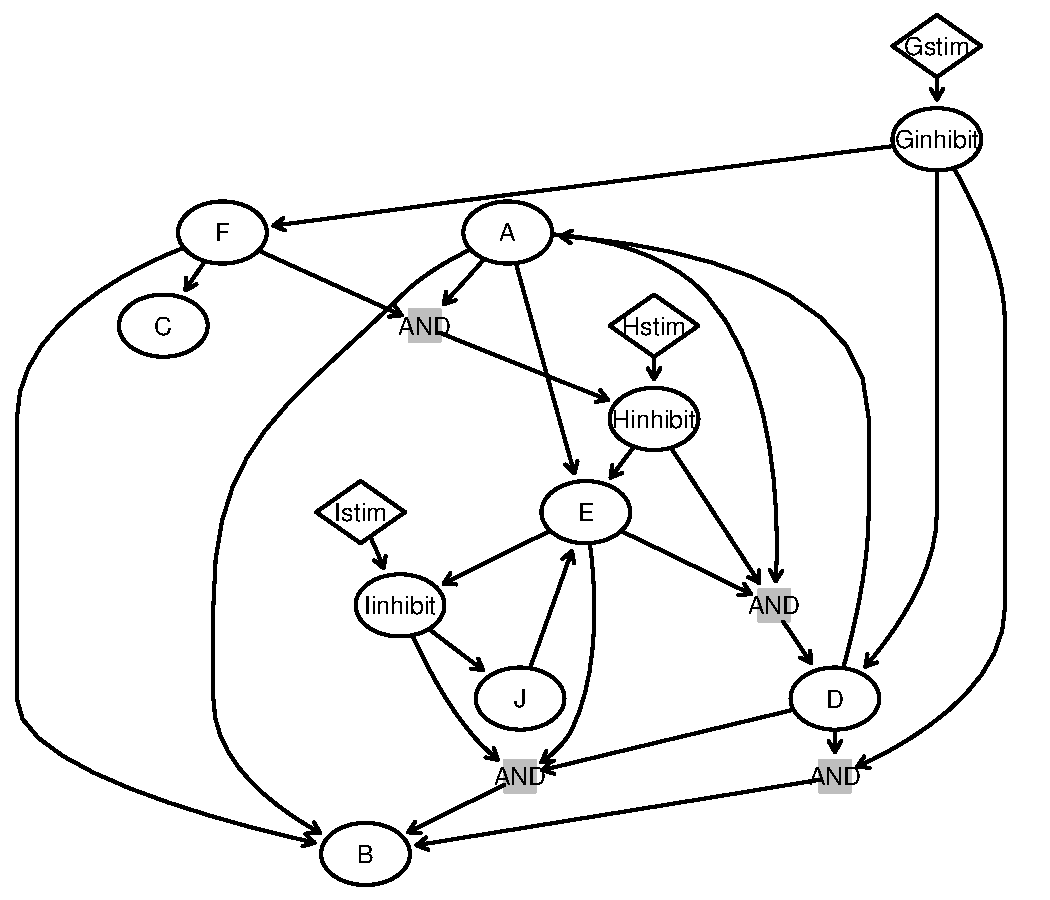
\includegraphics[width=0.6\linewidth]{figure/plotgtn2-1} 

}



\end{knitrout}
\begin{knitrout}
\definecolor{shadecolor}{rgb}{0.969, 0.969, 0.969}\color{fgcolor}\begin{kframe}
\begin{alltt}
\hlstd{exprs} \hlkwb{<-} \hlkwd{t}\hlstd{(steadyState)[}\hlkwd{rep}\hlstd{(}\hlnum{1}\hlopt{:}\hlkwd{ncol}\hlstd{(steadyState),} \hlnum{10}\hlstd{),} \hlkwd{rep}\hlstd{(}\hlnum{1}\hlopt{:}\hlkwd{nrow}\hlstd{(steadyState),} \hlnum{3}\hlstd{)]}
\hlstd{ERS} \hlkwb{<-} \hlkwd{computeFc}\hlstd{(CNOlist,} \hlkwd{t}\hlstd{(steadyState))}
\hlstd{stimuli.pairs} \hlkwb{<-} \hlkwd{apply}\hlstd{(}\hlkwd{apply}\hlstd{(}\hlkwd{expand.grid}\hlstd{(stimuli, stimuli),} \hlkwd{c}\hlstd{(}\hlnum{1}\hlstd{,}\hlnum{2}\hlstd{), as.character),} \hlnum{1}\hlstd{, paste,} \hlkwc{collapse} \hlstd{=} \hlstr{"_"}\hlstd{)}
\hlstd{ERS} \hlkwb{<-} \hlstd{ERS[,} \hlkwd{grep}\hlstd{(}\hlkwd{paste}\hlstd{(}\hlkwd{c}\hlstd{(}\hlkwd{paste}\hlstd{(}\hlstr{"Ctrl_vs_"}\hlstd{,} \hlkwd{c}\hlstd{(stimuli, inhibitors),} \hlkwc{sep} \hlstd{=} \hlstr{""}\hlstd{),} \hlkwd{paste}\hlstd{(stimuli,} \hlstr{"_vs_"}\hlstd{, stimuli,} \hlstr{"_"}\hlstd{,} \hlkwd{rep}\hlstd{(inhibitors,} \hlkwc{each} \hlstd{=} \hlkwd{length}\hlstd{(stimuli)),} \hlkwc{sep} \hlstd{=} \hlstr{""}\hlstd{),} \hlkwd{paste}\hlstd{(stimuli.pairs,} \hlstr{"_vs_"}\hlstd{, stimuli.pairs,} \hlstr{"_"}\hlstd{,} \hlkwd{rep}\hlstd{(inhibitors,} \hlkwc{each} \hlstd{=} \hlkwd{length}\hlstd{(stimuli.pairs)),} \hlkwc{sep} \hlstd{=} \hlstr{""}\hlstd{)),} \hlkwc{collapse} \hlstd{=} \hlstr{"|"}\hlstd{),} \hlkwd{colnames}\hlstd{(ERS))]}
\hlstd{fc} \hlkwb{<-} \hlstd{ERS[}\hlkwd{rep}\hlstd{(}\hlnum{1}\hlopt{:}\hlkwd{nrow}\hlstd{(ERS),} \hlnum{10}\hlstd{),} \hlkwd{rep}\hlstd{(}\hlnum{1}\hlopt{:}\hlkwd{ncol}\hlstd{(ERS),} \hlnum{3}\hlstd{)]}
\hlstd{fc} \hlkwb{<-} \hlstd{fc} \hlopt{+} \hlkwd{rnorm}\hlstd{(}\hlkwd{length}\hlstd{(fc),} \hlnum{0}\hlstd{,} \hlnum{1}\hlstd{)}
\hlstd{flip} \hlkwb{<-} \hlkwd{sample}\hlstd{(}\hlnum{1}\hlopt{:}\hlkwd{nrow}\hlstd{(fc),} \hlkwd{floor}\hlstd{(}\hlnum{0.33}\hlopt{*}\hlkwd{row}\hlstd{(fc)))}
\hlstd{fc[flip, ]} \hlkwb{<-} \hlstd{fc[flip, ]}\hlopt{*}\hlstd{(}\hlopt{-}\hlnum{1}\hlstd{)}
\hlkwd{rownames}\hlstd{(fc)} \hlkwb{<-} \hlkwd{paste}\hlstd{(}\hlkwd{rownames}\hlstd{(fc),} \hlnum{1}\hlopt{:}\hlkwd{nrow}\hlstd{(fc),} \hlkwc{sep} \hlstd{=} \hlstr{"_"}\hlstd{)}
\hlkwd{print}\hlstd{(fc[}\hlnum{1}\hlopt{:}\hlnum{6}\hlstd{,} \hlkwd{c}\hlstd{(}\hlnum{1}\hlopt{:}\hlnum{3}\hlstd{,(}\hlkwd{ncol}\hlstd{(fc)}\hlopt{-}\hlnum{2}\hlstd{)}\hlopt{:}\hlkwd{ncol}\hlstd{(fc))])}
\end{alltt}
\begin{verbatim}
##       Ctrl_vs_A  Ctrl_vs_B  Ctrl_vs_C Hstim_Istim_vs_Hstim_Istim_Hinhibit
## A_1 -0.78149795 -1.0243869 -0.4798684                           0.2478244
## B_2 -0.01482601 -1.5781127  0.1669494                           0.7255230
## C_3  0.76593851  2.6812805 -0.5003797                          -0.8308681
## D_4 -0.97604903 -0.2445900  1.7634378                           1.2054856
## E_5 -1.02583577  0.8197866  0.6801132                          -1.9870181
## F_6 -0.82180858  1.0003305  1.1556738                          -0.8102499
##     Hstim_Istim_vs_Hstim_Istim_Iinhibit Hstim_Istim_vs_Hstim_Istim_J
## A_1                         -1.09111396                   -0.1834281
## B_2                          2.19723830                    0.3406081
## C_3                         -0.02646857                    0.1008377
## D_4                         -0.86552369                   -0.3583840
## E_5                          0.76103492                   -0.4754561
## F_6                         -1.15428818                    1.2788998
\end{verbatim}
\end{kframe}
\end{knitrout}
\begin{knitrout}
\definecolor{shadecolor}{rgb}{0.969, 0.969, 0.969}\color{fgcolor}\begin{kframe}
\begin{alltt}
\hlstd{initBstring} \hlkwb{<-} \hlkwd{reduceGraph}\hlstd{(}\hlkwd{rep}\hlstd{(}\hlnum{0}\hlstd{,} \hlkwd{length}\hlstd{(model}\hlopt{$}\hlstd{reacID)), model, CNOlist)}
\hlstd{greedy2} \hlkwb{<-} \hlkwd{bnem}\hlstd{(}\hlkwc{search} \hlstd{=} \hlstr{"greedy"}\hlstd{,}
            \hlkwc{CNOlist}\hlstd{=CNOlist,}
            \hlkwc{fc}\hlstd{=fc,}
            \hlkwc{exprs}\hlstd{=exprs,}
            \hlkwc{model}\hlstd{=model,}
            \hlkwc{parallel}\hlstd{=parallel,}
            \hlkwc{initBstring}\hlstd{=initBstring,}
            \hlkwc{draw} \hlstd{=} \hlnum{FALSE}\hlstd{,}
            \hlkwc{verbose} \hlstd{=} \hlnum{FALSE}\hlstd{,}
            \hlkwc{maxSteps} \hlstd{=} \hlnum{Inf}
            \hlstd{)}
\end{alltt}


{\ttfamily\noindent\itshape\color{messagecolor}{\#\# snowfall 1.84-6.1 initialized (using snow 0.4-1): parallel execution on 2 CPUs.}}\begin{verbatim}
## Library CellNOptR loaded.
\end{verbatim}


{\ttfamily\noindent\itshape\color{messagecolor}{\#\# Library CellNOptR loaded in cluster.}}\begin{verbatim}
## Library bnem loaded.
\end{verbatim}


{\ttfamily\noindent\itshape\color{messagecolor}{\#\# Library bnem loaded in cluster.}}

{\ttfamily\noindent\itshape\color{messagecolor}{\#\# \\\#\# Stopping cluster}}\begin{alltt}
\hlstd{resString2} \hlkwb{<-} \hlstd{greedy2}\hlopt{$}\hlstd{bString}
\end{alltt}
\end{kframe}
\end{knitrout}
\begin{knitrout}
\definecolor{shadecolor}{rgb}{0.969, 0.969, 0.969}\color{fgcolor}\begin{kframe}
\begin{alltt}
\hlkwd{par}\hlstd{(}\hlkwc{mfrow}\hlstd{=}\hlkwd{c}\hlstd{(}\hlnum{1}\hlstd{,}\hlnum{2}\hlstd{))}
\hlkwd{plotDnf}\hlstd{(model}\hlopt{$}\hlstd{reacID[}\hlkwd{as.logical}\hlstd{(bString)],} \hlkwc{main} \hlstd{=} \hlstr{"GTN"}\hlstd{,} \hlkwc{stimuli} \hlstd{= stimuli)}
\end{alltt}
\begin{verbatim}
## A graphNEL graph with directed edges
## Number of Nodes = 17 
## Number of Edges = 28
\end{verbatim}
\begin{alltt}
\hlkwd{plotDnf}\hlstd{(model}\hlopt{$}\hlstd{reacID[}\hlkwd{as.logical}\hlstd{(resString2)],} \hlkwc{main} \hlstd{=} \hlstr{"greedy optimum"}\hlstd{,} \hlkwc{stimuli} \hlstd{= stimuli)}
\end{alltt}
\begin{verbatim}
## A graphNEL graph with directed edges
## Number of Nodes = 14 
## Number of Edges = 16
\end{verbatim}
\end{kframe}

{\centering 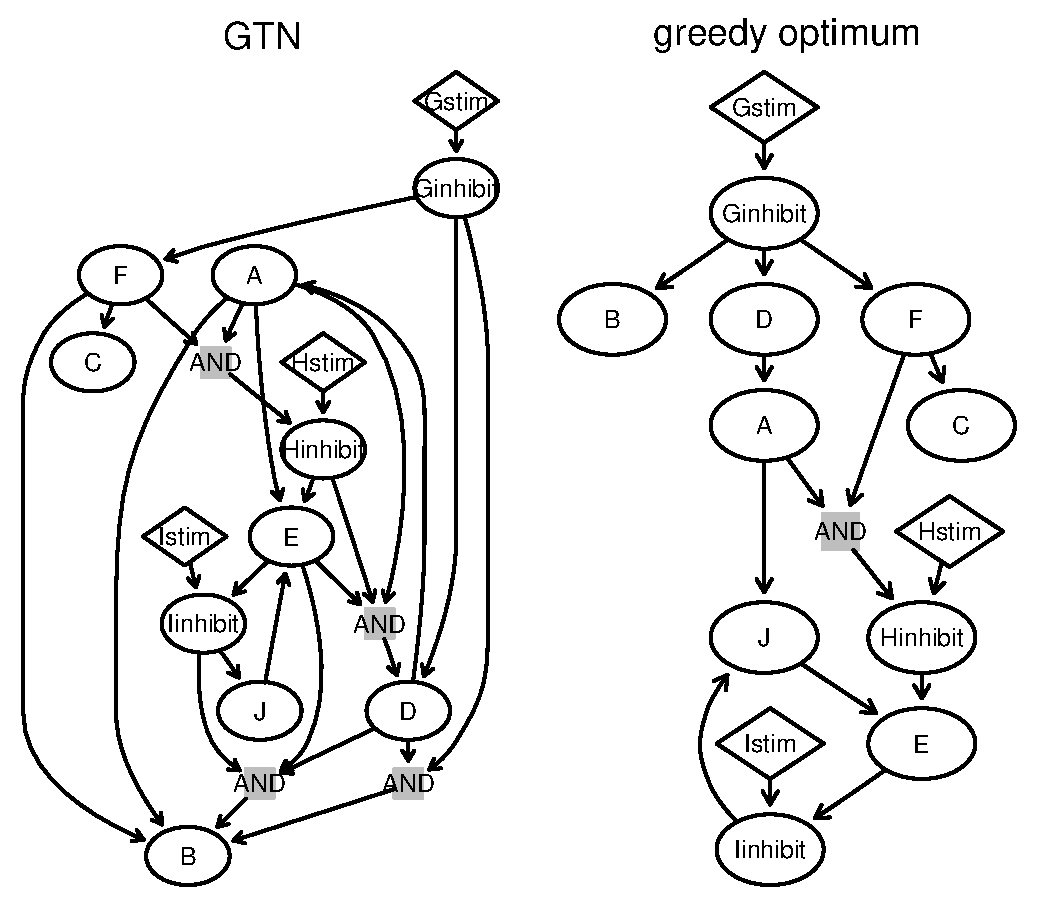
\includegraphics[width=0.6\linewidth]{figure/plotresult2-1} 

}



\end{knitrout}
\begin{knitrout}
\definecolor{shadecolor}{rgb}{0.969, 0.969, 0.969}\color{fgcolor}\begin{kframe}
\begin{alltt}
\hlkwd{print}\hlstd{(}\hlkwd{sum}\hlstd{(bString} \hlopt{==} \hlnum{1} \hlopt{&} \hlstd{resString2} \hlopt{==} \hlnum{1}\hlstd{)}\hlopt{/}\hlstd{(}\hlkwd{sum}\hlstd{(bString} \hlopt{==} \hlnum{1} \hlopt{&} \hlstd{resString2} \hlopt{==} \hlnum{1}\hlstd{)} \hlopt{+} \hlkwd{sum}\hlstd{(bString} \hlopt{==} \hlnum{1} \hlopt{&} \hlstd{resString2} \hlopt{==} \hlnum{0}\hlstd{)))}
\end{alltt}
\begin{verbatim}
## [1] 0.7222222
\end{verbatim}
\begin{alltt}
\hlkwd{print}\hlstd{(}\hlkwd{sum}\hlstd{(bString} \hlopt{==} \hlnum{0} \hlopt{&} \hlstd{resString2} \hlopt{==} \hlnum{0}\hlstd{)}\hlopt{/}\hlstd{(}\hlkwd{sum}\hlstd{(bString} \hlopt{==} \hlnum{0} \hlopt{&} \hlstd{resString2} \hlopt{==} \hlnum{0}\hlstd{)} \hlopt{+} \hlkwd{sum}\hlstd{(bString} \hlopt{==} \hlnum{0} \hlopt{&} \hlstd{resString2} \hlopt{==} \hlnum{1}\hlstd{)))}
\end{alltt}
\begin{verbatim}
## [1] 0.9912281
\end{verbatim}
\begin{alltt}
\hlstd{ERS.res} \hlkwb{<-} \hlkwd{computeFc}\hlstd{(CNOlist,} \hlkwd{t}\hlstd{(}\hlkwd{simulateStatesRecursive}\hlstd{(CNOlist, model, resString2)))}
\hlstd{ERS.res} \hlkwb{<-} \hlstd{ERS.res[,} \hlkwd{which}\hlstd{(}\hlkwd{colnames}\hlstd{(ERS.res)} \hlopt \hlkwd{colnames}\hlstd{(ERS))]}
\hlkwd{print}\hlstd{(}\hlkwd{sum}\hlstd{(ERS.res} \hlopt{==} \hlstd{ERS)}\hlopt{/}\hlkwd{length}\hlstd{(ERS))}
\end{alltt}
\begin{verbatim}
## [1] 1
\end{verbatim}
\end{kframe}
\end{knitrout}
The optimal network looks very different and has lower sensitivity and specificity. However the accuracy of the ERS is still $100\%$.
\begin{knitrout}
\definecolor{shadecolor}{rgb}{0.969, 0.969, 0.969}\color{fgcolor}\begin{kframe}
\begin{alltt}
\hlkwd{sessionInfo}\hlstd{()}
\end{alltt}
\begin{verbatim}
## R version 3.3.1 (2016-06-21)
## Platform: x86_64-apple-darwin13.4.0 (64-bit)
## Running under: OS X 10.11.5 (El Capitan)
## 
## locale:
## [1] C/UTF-8/C/C/C/C
## 
## attached base packages:
## [1] grid      parallel  stats     graphics  grDevices utils     datasets  methods  
## [9] base     
## 
## other attached packages:
##  [1] latticeExtra_0.6-28 RColorBrewer_1.1-2  lattice_0.20-33     bnem_1.0           
##  [5] snowfall_1.84-6.1   snow_0.4-1          matrixStats_0.50.2  nem_2.46.0         
##  [9] CellNOptR_1.18.0    XML_3.98-1.4        Rgraphviz_2.16.0    RCurl_1.95-4.8     
## [13] bitops_1.0-6        ggplot2_2.1.0       hash_2.2.6          RBGL_1.48.1        
## [17] graph_1.50.0        BiocGenerics_0.18.0 devtools_1.12.0     knitr_1.14         
## 
## loaded via a namespace (and not attached):
##  [1] Rcpp_0.12.6      formatR_1.4      git2r_0.15.0     highr_0.6        plyr_1.8.4      
##  [6] class_7.3-14     tools_3.3.1      boot_1.3-18      digest_0.6.10    statmod_1.4.25  
## [11] evaluate_0.9     memoise_1.0.0    gtable_0.2.0     curl_1.2         e1071_1.6-7     
## [16] withr_1.0.2      httr_1.2.1       stringr_1.0.0    stats4_3.3.1     R6_2.1.2        
## [21] plotrix_3.6-3    tcltk_3.3.1      limma_3.28.17    magrittr_1.5     scales_0.4.0    
## [26] colorspace_1.2-6 stringi_1.1.1    munsell_0.4.3
\end{verbatim}
\end{kframe}
\end{knitrout}

Pirkl, Martin, Hand, Elisabeth, Kube, Dieter, \& Spang, Rainer. 2016. Analyzing synergistic and non-synergistic interactions in signalling pathways using Boolean Nested Effect Models. \textit{Bioinformatics}, 32(6), 893–900.

\end{document}
